\section{Characterising Workflow Decay}
\label{sec:decay}

The main impediment to workflow preservation is workflow decay. Indeed, our experience with scientific workflows suggests that a large proportion of workflows suffer from decay \cite{DBLP:conf/eScience/Belhajjame07}, which decreases their value over time. Broadly speaking, we can distinguish two forms of decay. i)- {\bf Inability to re-execute the workflow}: due to many factors, including the unavailability of third party resources that are responsible for executing the tasks that compose the workflows, we may not be able to re-execute a given workflow. ii)- {\bf Inability to reproduce workflow results}: a less severe, yet relevant, form of decay, is the inability to obtain the same (or similar) results when re-executing the workflow. Reproducing previous results can be primordial in reinforcing trust in scientific results and can be used in peer-reviewing as a mechanism to validate the results claimed by given scientists \cite{DBLP:journals/pvldb/FreireBS11,carole2011}. 

The above discussion raises the following question. {\em What are the causes of workflow decay?} To identify and characterise the causes of workflow decay, we adopted a bottom-up approach, whereby we manually analyzed $92$ Taverna workflows from the myExperiment repository. We chose Taverna workflows because they form the largest available workflow collection (more than half of the workflows in myExperiment are Taverna workflows at the time of writing), and Taverna workflows have been published on myExperiment since its launch in 2007, therefore providing a good insight into decay over those years. 

To base our analysis on a sample of workflows that is representative of the set of workflows in myExperiment, we selected workflows using the following three criteria: 
\begin{itemize}
\item
The year of creation of the workflow: we believe that the decay of workflows could be directly impacted by the year of their creation, hence we tried to make an even coverage of Taverna 1 workflows \cite{DBLP:journals/bioinformatics/OinnAFMSGCGPWL04} and Taverna 2 workflows \cite{DBLP:conf/ssdbm/MissierSOTNDWOG10} between the years 2007 and 2012.
\item
The creator of the workflow:  in order to reduce possible bias introduced by specific workflow creators, we avoided choosing workflows created by the same person in the same year.
\item
The domain of the workflow: our workflow selection also had a good coverage of domains, covering $18$ different scientific (such as life sciences, astronomy and cheminformatics) and non-scientific domains (such as testing of Grid services).  Figures \ref{fig:domain_distribution} illustrates the domains of the workflows that we selected for decay analysis.
\end{itemize}
 
 \begin{figure}[h]
  \begin{center}
    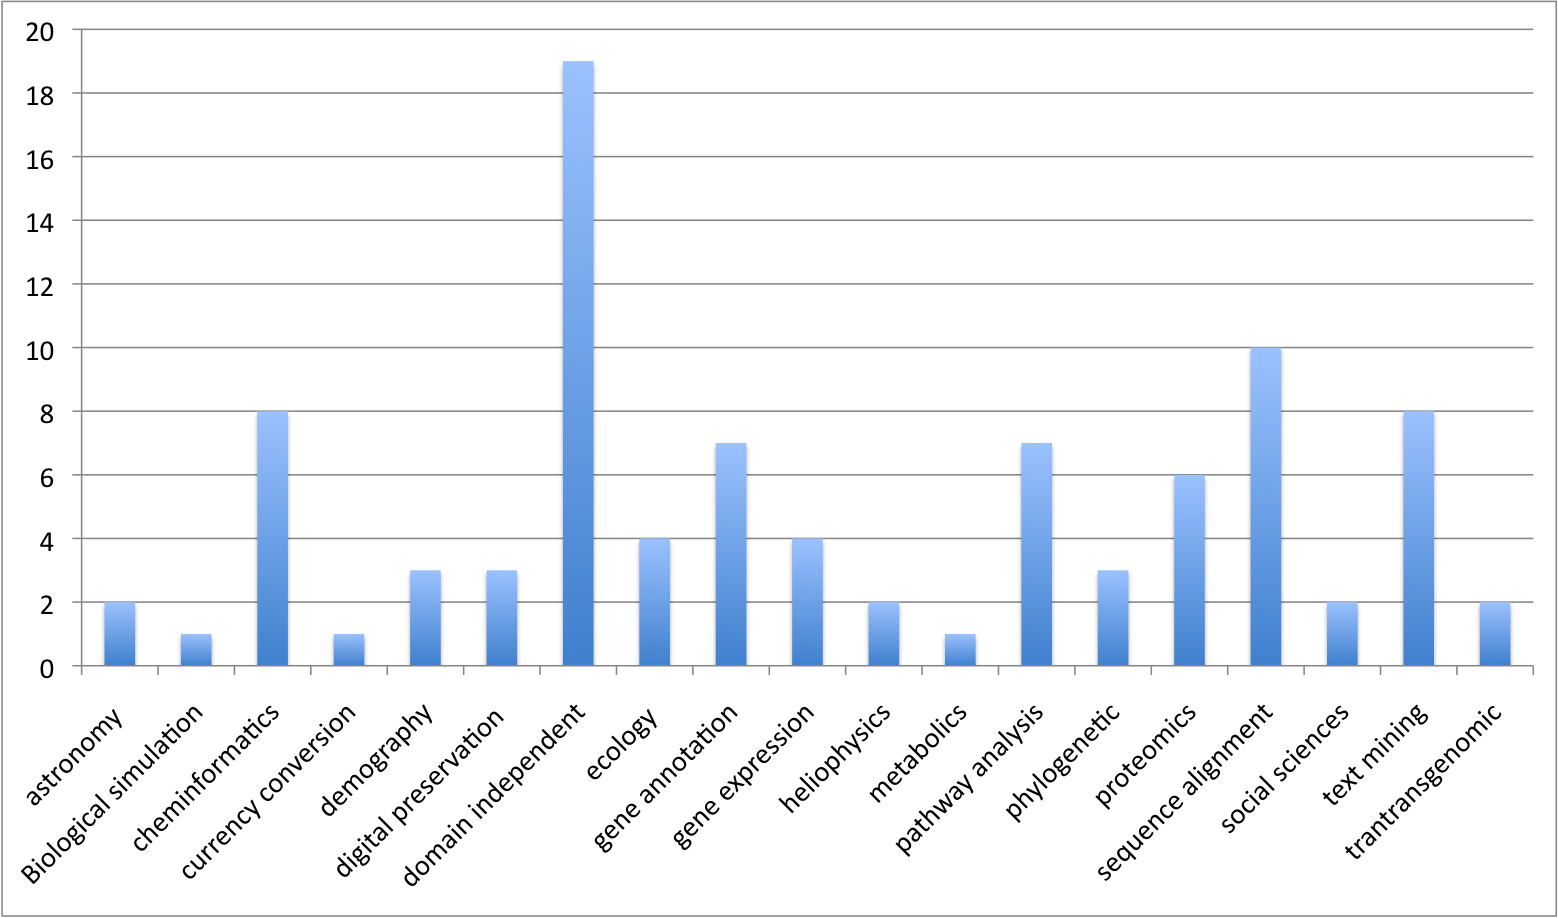
\includegraphics[width=13cm]{./Figures/domain-features.png}
        \caption{Distribution of the domain studied by our test workflows.}
        \label{fig:domain_distribution}
  \end{center}
\end{figure}


Although we focus on a particular family of workflows, i.e., Taverna workflows, we expect our approach and analysis to be applicable to many others and our analysis to be repeatable on a different corpus of workflows. 

To identify the causes of decay that the workflows we selected may suffer from, we attempted to execute them using the Taverna 2.3 workbench. We then manually examined their results, diagnosed broken links, etc. Our analysis showed that nearly $80\%$ of the tested workflows failed to be either executed or produce the same results, and those from earlier years (2007-2009) had more than 80\% failure rate (as shown in Figures~\ref{fig:taverna-wf-failed}). The causes of workflow decay can be classified into four categories, which we present in the rest of this section. 

% \begin{figure}[h]
%   \centering
%   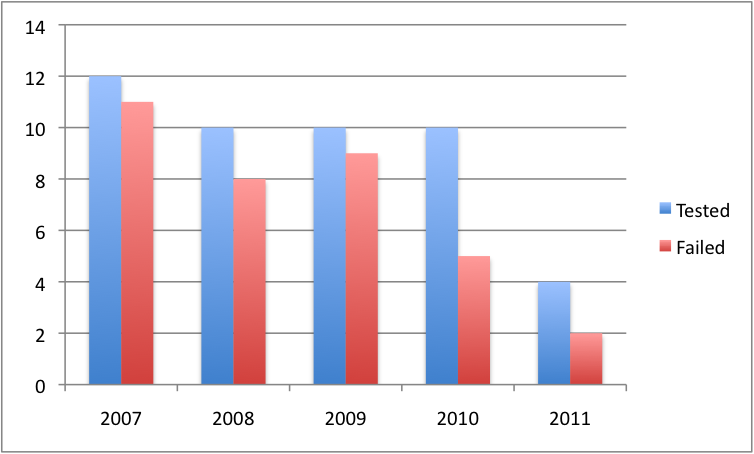
\includegraphics[width=7cm]{./Figures/taverna1-workflows-rate.png}
%   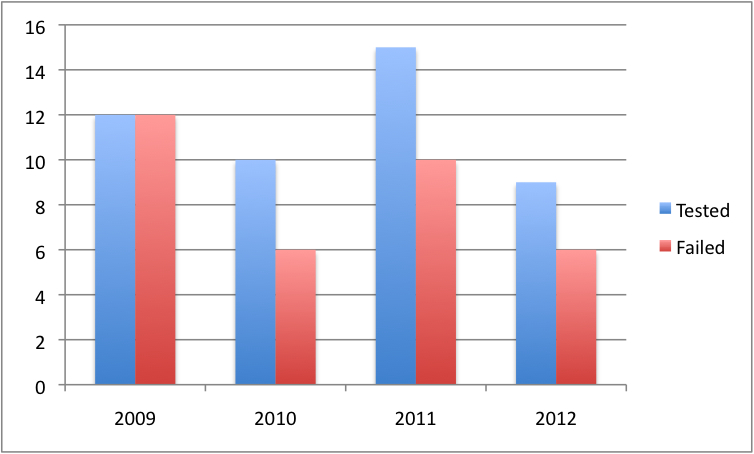
\includegraphics[width=7cm]{./Figures/taverna2-workflows-rate.png}
%  \caption{Number of Taverna workflows tested and failed (Taverna 1 on the left, Taverna 2 on the right)}
%  \label{fig:taverna-wf-failed}
% \end{figure}

\begin{figure}[h]
  \centering
  \begin{subfigure}[t]{8.25cm}
    \centering
    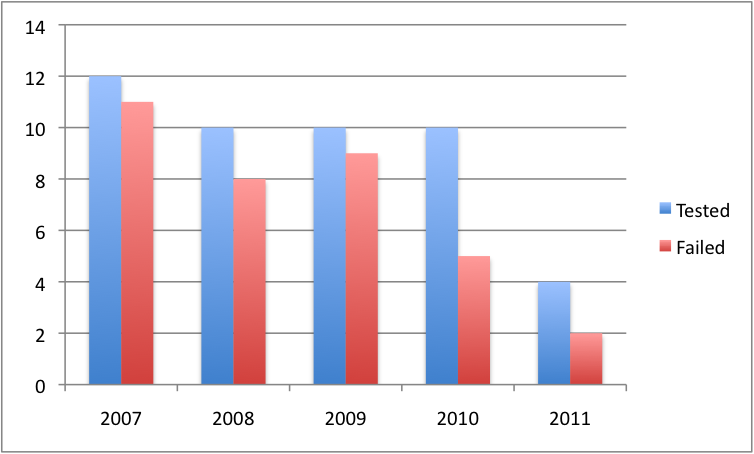
\includegraphics[width=8cm]{./Figures/taverna1-workflows-rate.png}
    \caption{Number of Taverna 1 workflows tested and failed.}
  \end{subfigure}
  \begin{subfigure}[t]{8.25cm}
    \centering
    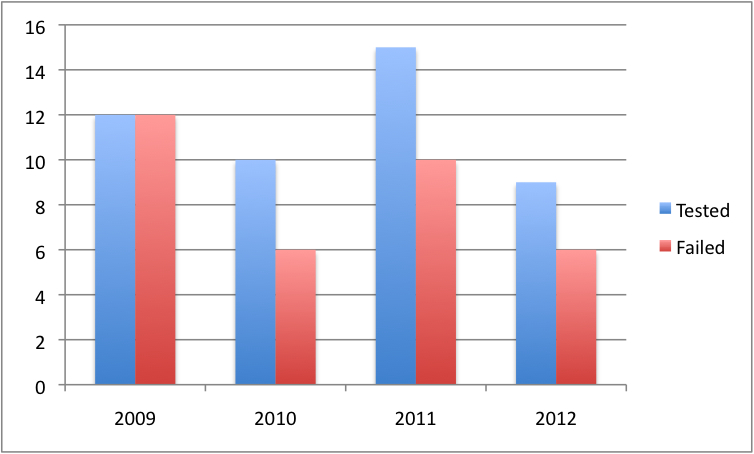
\includegraphics[width=8cm]{./Figures/taverna2-workflows-rate.png}
    \caption{Number of Taverna 2 workflows tested and failed.}
  \end{subfigure}
  \caption{Number of Taverna workflows tested and failed.}
  \label{fig:taverna-wf-failed}
\end{figure}

%   \begin{figure}[h]
%   \centering
%   \subfigure[Number of Taverna 1 workflows tested and failed.]{
%   	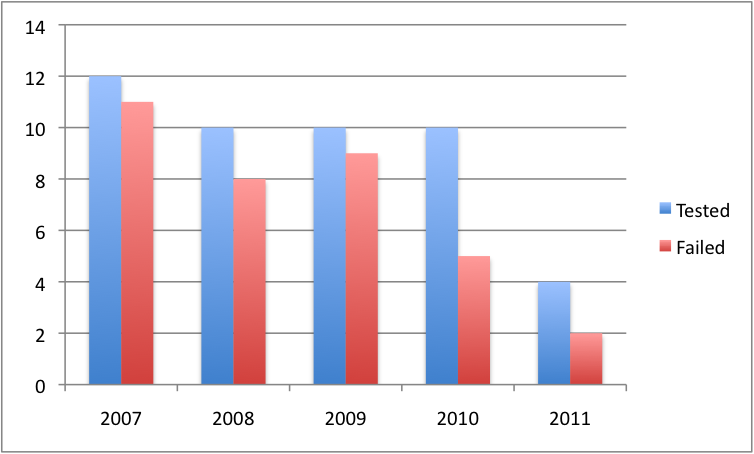
\includegraphics[width=7cm]{./Figures/taverna1-workflows-rate.png}}
%   \subfigure[Number of Taverna 2 workflows tested and failed.]{
%       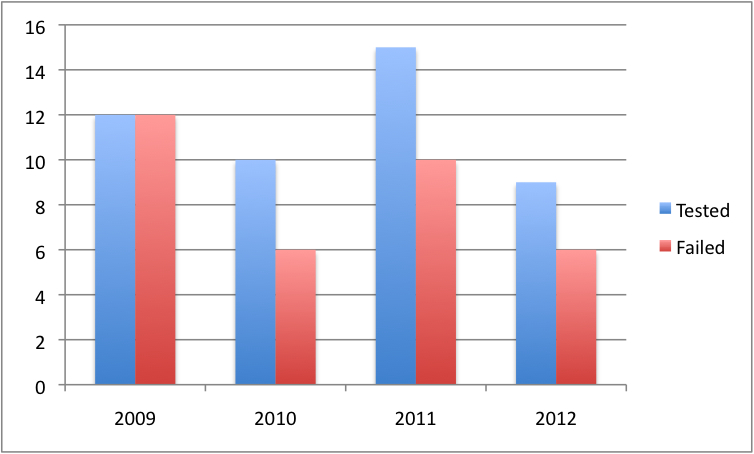
\includegraphics[width=7cm]{./Figures/taverna2-workflows-rate.png}}
%   \caption{Number of Taverna workflows tested and failed.}
%   \label{fig:taverna-wf-failed}
%   \end{figure}


\subsection{Volatile third-party resources}
Most of the workflows that we analysed make use of third-party resources such as web services and databases.
The provision of such resources may be interrupted or changed, causing failure of the workflow to execute. In certain cases, the workflow cannot be run, even when the third party resources that it relies on are available, e.g.,  when such resources require authentication. Another cause that may lead to workflow decay, is changes to third party resources. For example, if the web service provider decides to change the implementation of the web service, then the workflow execution may not deliver the same results, or worse, it may not be possible to execute. Table~\ref{table:decay} summarises these causes of decay with concrete examples.


\begin{table}[ht]
\caption{Categorisation of Decay Caused by Third-party Resources} % title of Table
\centering  % used for centering table
\begin{tabular}{p{1.6in} p{2.2in} p{2.2in}} % centered columns (4 columns)
\hline\hline                        %inserts double horizontal lines
Causes &  Refined causes & Examples \\
\hline                  

Third party resources are not available & Underlying datasets, particularly those locally hosted in-house datasets, are no longer available & Researcher hosting the data changed institution, server is no longer available 
\\ \cline{2-3} 
			 									& Services are deprecated & (DNA Data Bank of Japan) DDBJ web services are not longer provided despite the fact that they are used in many myExperiment workflows
 \\ \hline

Third party resources are available but not accessible & Data is available but identified using different IDs than the one known to the user & Due to scalability reasons the input data is superseded by a new version making the workflow not executable or providing wrong results
\\ \cline{2-3}

								& Data is available but permission, certificate, or network to access it is needed & Cannot get the input, which is a security token that can only be obtained by a registered user of ChemiSpider
\\ \cline{2-3}
								& Services are available but need permission, certificate, or network to access and invoke them	& The security policies of the execution framework are updated due to new hosting institution rules \\
\hline
Third party resources have changed &  Services are still available by using the same identifiers but their functionality have changed & The web services are updated intentionally or unintentionally (e.g.malware) providing wrong results \\
\hline
\end{tabular}
\label{table:decay} % is used to refer this table in the text
\end{table}

\subsection{Missing example data}
It is not always obvious which data can be used as inputs to the workflow execution, and example inputs are often helpful.  Example outputs can also be useful to gain an insight of the outcome anticipated from the workflow. However, our analysis revealed that they are not always made available. Provenance traces of previous runs are also useful as indications of where example data may be found.


\subsection{Missing execution environment}
The execution of a workflow may rely on a particular local execution environment, for example, a local R server or a specific version of workflow execution software. Some of our test workflows exhibit this type of decay. Taverna often provides sufficient information about missing libraries, and sometimes workflow descriptions provide a warning about the requirement for a specific library. This type of decay appears to be fixable by installing the missing software, albeit requiring some effort.

\subsection{Insufficient descriptions about workflows}
Sometimes a workflow workbench cannot provide sufficient information about what caused the failure of a workflow run. Additional descriptions in the workflow can play an important role in assisting re-users to understand the purpose of the workflow and its expected outcomes.



The results of the above analysis are summarised in Figure \ref{fig:decay-analysis}-a, which illustrates the number of workflows that suffer from each of the causes of decay presented above. It shows that {50\%} workflows suffer from decay due to third party resources. 

\begin{figure}[ht]
\centering
\begin{subfigure}[t]{8.25cm}
  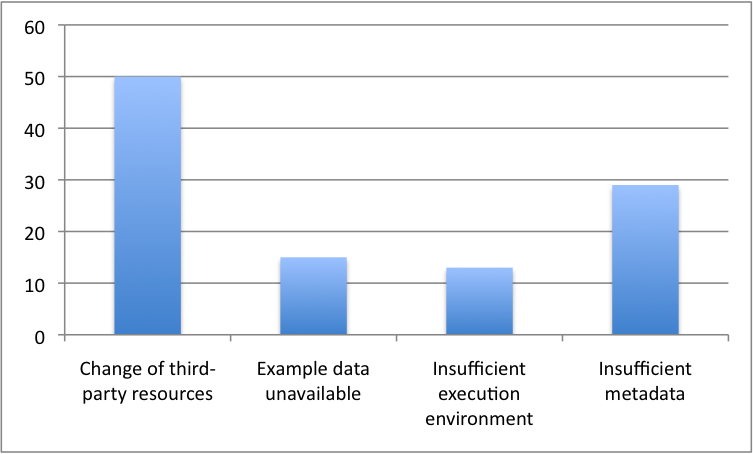
\includegraphics[width=8cm]{./Figures/decay_analysis_chart1-v2.png}
  \caption{A summary of workflow decay causes}
\end{subfigure}
\begin{subfigure}[t]{8.25cm}
  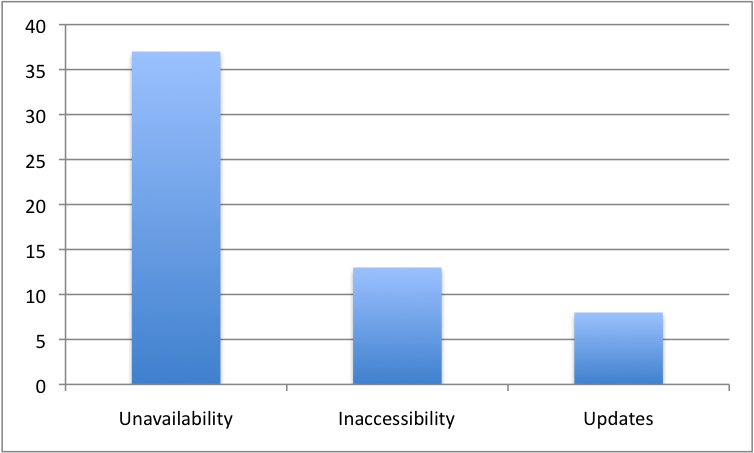
\includegraphics[width=8cm]{./Figures/decay_analysis_chart2-v2.png}
  \caption{Workflow decay due to third party resources}
\end{subfigure}
\caption{Results of workflow decay analysis.}
\label{fig:decay-analysis}
\end{figure}


% \begin{figure}[ht]
% \centering
% \subfigure[A summary of workflow decay causes.]{
% 	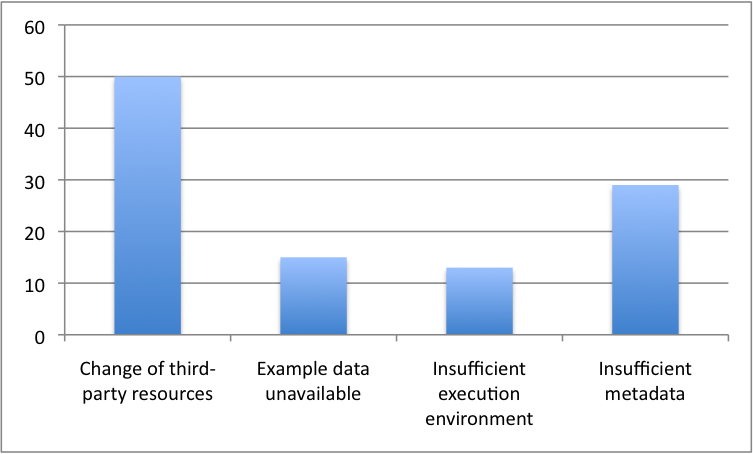
\includegraphics[width=9cm]{./Figures/decay_analysis_chart1-v2.png}
% }
% \subfigure[Workflow decay due to third party resources.]{
%     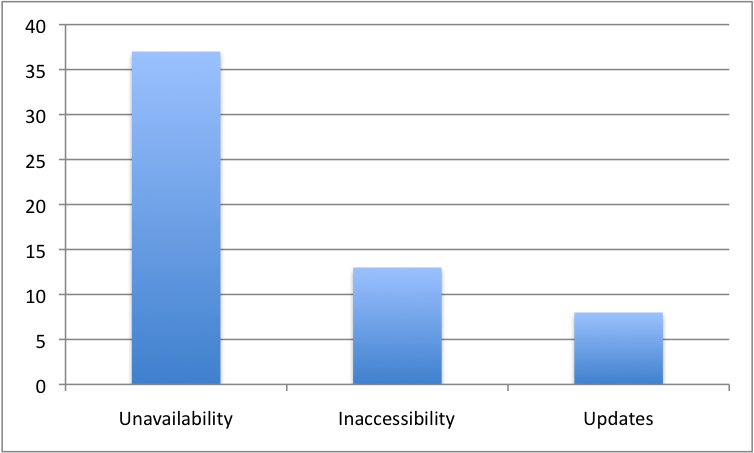
\includegraphics[width=7cm]{./Figures/decay_analysis_chart2-v2.png}
% }
% \caption{Results of workflow decay analysis.}
% \label{fig:decay-analysis}
% \end{figure}


To better understand the causes of decay due to third party resources. Figure \ref{fig:decay-analysis}-b illustrates the number of workflows that suffer from the causes presented in Table~\ref{table:decay}. It shows that the unavailability of third party resources is the leading cause of decay, followed by resources inaccessibility, and then resources changes. 

The above results confirms our hypothesis that workflow decay is a serious problem. It also suggests that there is a need for additional information that can assist workflow designers detecting and repairing decayed workflows. We report in a separate deliverable \cite{D4.2v1}, on a minimal model and associated checklists, that were designed and developed with the objective to prevent and repair workflow decay.
